
\begin{multicols}{2}
Pour une épreuve d'orientation, Aurore reçoit
le plan ci-contre. Sachant que les droites $(EF)$ et $(IA)$ sont
parallèles ainsi que les droites $(GH)$ et $(DA)$, quelle est la
longueur du parcours $DEFGHA$ ?

\vspace{5mm}

$D$ : Départ\kern1cm $A$ : arrivée.\\
$DA=600$~m; $DE=200$~m; $IG=90$~m; $DI=315$~m; $IA=390$~m.

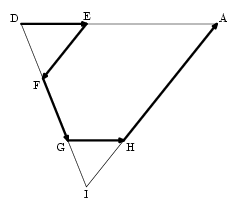
\includegraphics[scale=1]{TR-exo18.png} 

\end{multicols}